\documentclass[11pt,a4paper]{article}

% === Packages ===
\usepackage[utf8]{inputenc}
\usepackage[T1]{fontenc}
\usepackage{amsmath,amssymb,amsthm}
\usepackage{mathtools}
\usepackage{bm}
\usepackage{graphicx}
\usepackage[colorlinks=true,linkcolor=blue,citecolor=blue,urlcolor=blue]{hyperref}
\usepackage{natbib}
\usepackage{booktabs}
\usepackage{tabularx}
\usepackage{float}
\usepackage{caption}
\usepackage{subcaption}
\usepackage[margin=1in]{geometry}
\usepackage{tcolorbox}
\usepackage{enumitem}
\usepackage{xcolor}

% === Theorem environments ===
\newtheorem{theorem}{Theorem}[section]
\newtheorem{proposition}[theorem]{Proposition}
\newtheorem{lemma}[theorem]{Lemma}
\newtheorem{corollary}[theorem]{Corollary}
\theoremstyle{definition}
\newtheorem{definition}[theorem]{Definition}
\newtheorem{remark}[theorem]{Remark}

% === Boxed environments ===
\newtcolorbox{formalbox}[1][]{
  colback=blue!3,
  colframe=blue!40!black,
  fonttitle=\bfseries,
  title=#1,
  arc=2mm,
  boxrule=0.5mm,
}

\newtcolorbox{opbox}[1][]{
  colback=green!3,
  colframe=green!40!black,
  fonttitle=\bfseries,
  title=#1,
  arc=2mm,
  boxrule=0.5mm,
}

% === Notation shortcuts ===
\newcommand{\E}{\mathbb{E}}
\newcommand{\KL}{\mathrm{D}_{\mathrm{KL}}}
\newcommand{\R}{\mathbb{R}}
\newcommand{\bq}{q}
\newcommand{\bp}{p}
\newcommand{\bo}{\bm{o}}
\newcommand{\bs}{\bm{s}}
\newcommand{\ba}{\bm{a}}
\newcommand{\bpi}{\bm{\pi}}
\newcommand{\bmu}{\bm{\mu}}
\newcommand{\bbeta}{\bm{\beta}}
\newcommand{\bsigma}{\bm{\sigma}}
\newcommand{\boldeta}{\bm{\eta}}

% === Title ===
\title{
\textbf{The Semiotic Fabric as Cognitive Substrate:\\
Decentralized Active Inference Through Nested Markov Blankets\\
in Ultra-Large-Scale Data Architecture}
}

\author{
Mahault Albarracin$^{1,2,3}$ \and
S. Yoakum-Stover$^{4}$ \and
M. A. Eick$^{4}$ \and
Maxwell J. D. Ramstead$^{2,5}$ \and
Karl J. Friston$^{2,5}$
\\[6pt]
\small $^{1}$D\'{e}partement d'informatique, Universit\'{e} du Qu\'{e}bec \`{a} Montr\'{e}al, Canada \\
\small $^{2}$VERSES Research Lab, Los Angeles, CA, USA \\
\small $^{3}$Spatial Web Foundation, Los Angeles, CA, USA \\
\small $^{4}$Mission Focus, McLean, VA, USA \\
\small $^{5}$Wellcome Centre for Human Neuroimaging, University College London, UK
}

\date{March 2026}

\begin{document}

\maketitle

% ============================================================
% ABSTRACT
% ============================================================
\begin{abstract}
We argue that the SemApp semiotic data fabric --- an operational, petabyte-scale data architecture deployed within the U.S.\ Intelligence Community --- constitutes a cognitive substrate in the formal sense defined by the Free Energy Principle.
We establish a structural isomorphism between C.~S.~Peirce's triadic semiotics and variational inference, showing that SemApp's Sign Representation Framework implements semiosis as free energy minimization.
We prove that SemApp's three-layer data architecture (unstructured data, structured Signs, domain models) instantiates nested Markov blankets, with each layer satisfying the conditional independence requirements of the blanket partition.
We formalize Process Waves as active inference agents whose expected free energy decomposes into deontic, epistemic, and pragmatic components mapped to concrete SemApp operations.
We introduce the material free energy $\mathcal{F}_{\text{material}}$ of the fabric as a whole, showing that cumulative Wave processing monotonically decreases this quantity under consistent domain models.
A computational demonstration using \texttt{pymdp} validates the formal mapping through three experiments: single-Wave epistemic foraging on a semiotic grid, multi-Wave cooperation dynamics, and multi-scale free energy minimization across nested blanket levels.
These results establish that a semiotic data fabric organized into nested Markov blankets, with decentralized active inference agents operating over meaningful Signs, satisfies the formal criteria for cognition under the Free Energy Principle --- providing both explanatory power for why SemApp works at scale and predictive power for next-generation data architecture design.

\vspace{6pt}
\noindent\textbf{Keywords:} Active inference, Free Energy Principle, Markov blankets, semiotics, data fabric, Peircean signs, distributed cognition, ultra-large-scale systems, process waves, variational inference
\end{abstract}

\newpage
\tableofcontents
\newpage

% ============================================================
% 1. INTRODUCTION
% ============================================================
\section{Introduction}

\subsection{The Intelligence Problem in Ultra-Large-Scale Data Environments}
\label{sec:uls}

The national defense enterprise of the United States has a data problem. Despite spending billions annually on data collection, storage, processing, and management, the Intelligence Community (IC) and Department of Defense (DoD) struggle to capitalize on those investments \citep{sei2006uls, yoakumstover2025semapp}. The consequences to national security are serious: intelligence and military operations are impeded as basic command challenges go unmet.

The root cause, as identified by the Software Engineering Institute's landmark study \citep{sei2006uls}, is that the defense data ecosystem constitutes an \emph{Ultra-Large-Scale} (ULS) system --- characterized by decentralization, inherently conflicting requirements, heterogeneous elements, normal failures, continuous evolution, and immense scale along many dimensions. ULS systems are to ordinary systems as cities are to buildings: qualitatively different in kind, not merely in degree.

Traditional approaches to data unification --- \emph{harmonization} (merging data models into a canonical form) and \emph{federation} (translating through adapters to a canonical model) --- both fail at ULS scale because they attempt to impose a single semantic perspective on inherently diverse data. There is no one right way to represent all knowledge that will suffice for every purpose. To impose one destroys the essential complexity that gives intelligence its richness \citep{yoakumstover2025semapp}.

The conundrum is this: unifying data means having one interface to all data, which implies a single data model, entailing a single fixed perspective. But there is no one right way to represent all knowledge, and to impose one thwarts the ULS nature of the problem.

This paper proposes that this conundrum dissolves when viewed through the lens of active inference and the Free Energy Principle (FEP). The data problem is not merely an engineering challenge --- it is a \emph{cognitive} challenge. At ULS scale, a data system must \emph{make sense} of its contents: discovering patterns, resolving ambiguities, maintaining coherent representations while accommodating diversity. These are precisely the functions that the FEP attributes to cognitive systems.

We argue that the SemApp data fabric, developed by Mission Focus and operational on classified IC networks processing nearly 70 petabytes of diverse data \citep{yoakumstover2025semapp}, resolves this conundrum because --- whether by design or convergent evolution --- it has the architecture of a cognitive system. Specifically, it implements decentralized active inference through nested Markov blankets over a semiotic substrate.

\subsection{Active Inference as the Physics of Intelligence}
\label{sec:aif_intro}

The Free Energy Principle (FEP) provides a first-principles account of why self-organizing systems persist and how they maintain their identity in a changing world \citep{friston2019particular}. At its core, the FEP states that any system that maintains a boundary between itself and its environment --- formally, a \emph{Markov blanket} --- must minimize an information-theoretic quantity called \emph{variational free energy}. This minimization is equivalent to performing approximate Bayesian inference: the system implicitly maintains a model of its environment and acts to confirm its predictions.

Active inference extends this principle to agents that can act on their environment \citep{parr2022active}. Under active inference, perception is inference about the causes of sensory data, learning is inference about model parameters, and action is inference about the best policy --- the course of action that will minimize expected future surprise. The framework naturally decomposes action selection into epistemic (information-seeking) and pragmatic (goal-directed) components, providing a unified account of curiosity, exploration, and exploitation.

Crucially, the FEP is \emph{scale-free}: the same principles apply at every level of organization, from molecular interactions to neural circuits to social groups \citep{friston2019particular, kirchhoff2018markov, ramstead2023inner}. When a system contains subsystems that themselves have Markov blankets, these blankets \emph{nest}, creating a hierarchical architecture in which each level performs its own active inference while serving as a component of the level above. This multi-scale self-organization is what distinguishes genuinely cognitive systems from merely physical ones \citep{kirchhoff2018markov}.

Recent work has proposed that these principles can guide the design of ecosystems of natural and artificial intelligence \citep{friston2022ecosystems}. Rather than building monolithic AI systems, one can engineer distributed networks of intelligent agents that coordinate through shared generative models, forming emergent collective intelligence at superordinate scales. The substrate for this coordination --- the shared medium through which agents exchange beliefs and observations --- is what we identify with the semiotic data fabric.

\subsection{The Peircean Bridge: Semiotics Meets Statistical Physics}
\label{sec:peirce_intro}

The missing link between data architecture and cognitive science is \emph{semiotics} --- the study of signs and meaning-making. C.~S.~Peirce's triadic semiotics describes meaning as an inferential process: a \emph{sign} (representamen) stands for an \emph{object} (referent) to produce an \emph{interpretant} (meaning) in the mind of an interpreter \citep{peirce1931collected}. Critically, this is not a static relation but a \emph{process} --- \emph{semiosis} --- in which each interpretant becomes a new sign, generating unlimited chains of meaning.

Recent work in active inference has established a formal isomorphism between Peircean semiosis and variational inference \citep{constant2019regimes, ramstead2016cultural, albarracin2022epistemic}. The sign maps to an observation, the object maps to a hidden state, and the interpretant maps to the updated posterior belief. Semiosis --- the generation of meaning from signs --- \emph{is} variational inference, described in a different vocabulary.

This isomorphism is not merely an analogy. As \citet{albarracin2025nonmarkovian} argue, meaning and context are inherently non-Markovian: the interpretation of a sign depends on the full history of prior interpretations. The FEP accommodates this through temporal depth in generative models and through the non-Markovian dynamics that arise when systems maintain identity over time.

SemApp's fundamental data primitive --- the \emph{Sign}, which binds a \emph{Signifier} (data value) with a \emph{Concept} (meaning) --- is a computational implementation of Peirce's triadic sign. This paper formalizes this connection and shows that SemApp's entire architecture can be understood as a system performing active inference over semiotic content.

\subsection{Contributions and Paper Overview}
\label{sec:contributions}

This paper makes the following contributions:

\begin{enumerate}[label=(\roman*)]
    \item We establish a \textbf{formal isomorphism} between Peircean semiosis and variational inference (Theorem~\ref{thm:semiotic_fe}), showing that Sign creation in SemApp minimizes semiotic free energy.

    \item We prove that SemApp's \textbf{three-layer architecture constitutes nested Markov blankets} (Theorem~\ref{thm:nested_blanket}), with conditional independence holding between Artifacts (external states), Signs (blanket states), and domain models (internal states).

    \item We formalize \textbf{Process Waves as active inference agents} (Definition~\ref{def:wave_gm}) and show that the DEEP value decomposition \citep{constant2019regimes} maps onto concrete SemApp operations.

    \item We introduce the \textbf{material free energy} $\mathcal{F}_{\text{material}}$ of the fabric (Definition~\ref{def:f_material}) and show its monotonic decrease under consistent Wave processing (Proposition~\ref{prop:monotone}).

    \item We provide a \textbf{computational demonstration} using \texttt{pymdp} \citep{heins2022pymdp} that validates the formal mapping through three experiments on a simulated semiotic fabric.
\end{enumerate}

The paper is structured as follows. Section~\ref{sec:background} presents the theoretical foundations: the FEP, Peircean semiotics, and SemApp's architecture. Section~\ref{sec:formal} develops the formal mapping --- the mathematical core of the paper. Section~\ref{sec:fmaterial} introduces the material free energy framework. Section~\ref{sec:simulation} presents the computational demonstration. Section~\ref{sec:implications} discusses implications for both active inference theory and defense data architecture. Section~\ref{sec:discussion} addresses limitations and future directions. Section~\ref{sec:conclusion} concludes.

\begin{opbox}[Note to readers]
This paper serves two communities. For readers from the active inference and cognitive science community, the novel contribution is the mapping of FEP concepts onto a production-scale data architecture. For readers from the defense and intelligence community, the novel contribution is a theoretical framework that explains \emph{why} SemApp works and predicts \emph{how} to make it work better. Mathematical content is presented in blue boxes that can be skipped on a first reading without losing the narrative thread. Green boxes like this one provide operational implications.
\end{opbox}


% ============================================================
% 2. BACKGROUND AND THEORETICAL FOUNDATIONS
% ============================================================
\section{Background and Theoretical Foundations}
\label{sec:background}

\subsection{The Free Energy Principle and Active Inference}
\label{sec:fep}

\subsubsection{Variational Free Energy and the Generative Model}
\label{sec:vfe}

The Free Energy Principle begins with a simple observation: things that exist must, by definition, maintain their existence --- they must resist the tendency toward disorder mandated by the second law of thermodynamics. Any system that persists in a characteristic set of states can be described as if it possesses a boundary --- a \emph{Markov blanket} --- that separates its internal states from external states, and as if its internal dynamics implement a \emph{generative model} of how its sensory observations are caused by external states \citep{friston2019particular}.

\begin{formalbox}[Definition 1: Variational Free Energy]
Let $\bo$ denote observations (sensory states), $\bs$ denote hidden states of the environment, $\bq(\bs)$ denote an approximate posterior distribution (the system's beliefs about hidden states), and $\bp(\bo, \bs)$ denote a generative model (the system's model of how observations arise from hidden states). The \textbf{variational free energy} is:
\begin{equation}
\label{eq:vfe}
\mathcal{F} = \E_{\bq(\bs)}\!\left[\ln \bq(\bs) - \ln \bp(\bo, \bs)\right] = \underbrace{\KL\!\left[\bq(\bs) \,\|\, \bp(\bs|\bo)\right]}_{\geq\, 0} - \underbrace{\ln \bp(\bo)}_{\text{log evidence}}
\end{equation}
Since the KL divergence is non-negative, $\mathcal{F} \geq -\ln \bp(\bo)$. Minimizing $\mathcal{F}$ with respect to $\bq$ therefore simultaneously:
\begin{itemize}[nosep]
    \item Makes the approximate posterior $\bq(\bs)$ approach the true posterior $\bp(\bs|\bo)$ (perception)
    \item Maximizes a lower bound on the log model evidence $\ln \bp(\bo)$ (self-evidencing)
\end{itemize}
The generative model factorizes as:
\begin{equation}
\label{eq:gm}
\bp(\bo, \bs) = \underbrace{\bp(\bo|\bs)}_{\text{likelihood}} \cdot \underbrace{\bp(\bs)}_{\text{prior}}
\end{equation}
\end{formalbox}

In the discrete-state active inference framework \citep{parr2022active}, the generative model is parameterized by four sets of matrices:
\begin{itemize}[nosep]
    \item $\mathbf{A}$: likelihood mapping $\bp(\bo|\bs)$ --- how hidden states generate observations
    \item $\mathbf{B}$: transition dynamics $\bp(\bs_{t+1}|\bs_t, \ba_t)$ --- how states evolve under actions
    \item $\mathbf{C}$: log-preferences $\ln \bp(\bo)$ --- what observations the agent expects/prefers
    \item $\mathbf{D}$: initial state priors $\bp(\bs_0)$ --- beliefs about the starting state
\end{itemize}
These matrices fully specify an agent's generative model and are the objects we will map onto SemApp's architecture.

\subsubsection{Expected Free Energy and the DEEP Decomposition}
\label{sec:efe}

Active inference extends perception to action: an agent selects policies (sequences of actions) $\bpi$ that minimize \emph{expected free energy} --- the free energy the agent expects to encounter in the future if it follows a given policy.

\begin{formalbox}[Definition 2: Expected Free Energy and DEEP Decomposition]
The \textbf{expected free energy} of a policy $\bpi$ at future time $\tau$ is:
\begin{equation}
\label{eq:efe}
G(\bpi, \tau) = \E_{\tilde{\bq}}\!\left[\ln \bq(\bs_\tau | \bpi) - \ln \bp(\bo_\tau, \bs_\tau)\right]
\end{equation}
where $\tilde{\bq} = \bq(\bo_\tau, \bs_\tau | \bpi)$ is the predicted joint distribution over future observations and states under policy $\bpi$. This decomposes into:
\begin{equation}
\label{eq:deep}
G(\bpi, \tau) = \underbrace{-\E_{\tilde{\bq}}\!\left[\ln \bp(\bo_\tau)\right]}_{\text{Pragmatic value}} + \underbrace{-\E_{\tilde{\bq}}\!\left[\mathcal{H}\!\left[\bp(\bo_\tau|\bs_\tau)\right]\right]}_{\text{Epistemic value (ambiguity)}}
\end{equation}
Following \citet{constant2019regimes}, the expected free energy further decomposes into DEEP components:
\begin{itemize}[nosep]
    \item \textbf{D}eontic: value from conforming to environmental norms and deontic cues
    \item \textbf{E}pistemic: information gain about hidden states (resolving uncertainty)
    \item \textbf{E}xtrinsic/Pragmatic: achieving preferred outcomes
    \item \textbf{P}referential: fulfilling prior preferences about observations
\end{itemize}
An agent selects the policy that minimizes total expected free energy:
\begin{equation}
\label{eq:policy}
\bpi^* = \arg\min_{\bpi} \sum_{\tau} G(\bpi, \tau)
\end{equation}
\end{formalbox}

\begin{opbox}[Operational Implication]
The DEEP decomposition will map directly onto SemApp operations: Deontic value corresponds to classification and access control compliance; Epistemic value to query and discovery operations; Pragmatic value to enrichment and mission objectives; Preferential value to domain model conformance.
\end{opbox}

\subsubsection{Nested Markov Blankets and Multi-Scale Self-Organization}
\label{sec:nested_blankets}

A Markov blanket formalizes the boundary of a ``thing'' --- the minimal set of states that renders a system's internal states conditionally independent of its external environment.

\begin{formalbox}[Definition 3: Markov Blanket Partition]
A system's state space $\mathcal{X}$ admits a \textbf{Markov blanket partition} if it can be decomposed as:
\begin{equation}
\label{eq:blanket}
\mathcal{X} = \bmu \cup \bs \cup \ba \cup \boldeta
\end{equation}
where $\bmu$ are \emph{internal states}, $\bs$ are \emph{sensory states}, $\ba$ are \emph{active states}, and $\boldeta$ are \emph{external states}, such that:
\begin{equation}
\label{eq:ci}
\bp(\bmu, \boldeta \,|\, \bs, \ba) = \bp(\bmu \,|\, \bs, \ba) \cdot \bp(\boldeta \,|\, \bs, \ba)
\end{equation}
The \emph{blanket states} $\mathcal{B} = \bs \cup \ba$ mediate all statistical dependencies between internal and external states. External states influence internal states only through sensory states; internal states influence external states only through active states.
\end{formalbox}

The crucial insight of \citet{friston2019particular} is that Markov blankets \emph{nest}: if a system has a Markov blanket, and its internal states themselves admit Markov blanket partitions, then one obtains a recursive, hierarchical structure. At each level, the same active inference dynamics operate --- perception, action, and free energy minimization --- while the whole system self-organizes into a multi-scale cognitive architecture \citep{kirchhoff2018markov, ramstead2023inner}.

This nesting is not optional or decorative. As \citet{kirchhoff2018markov} argue in ``The Markov Blankets of Life,'' the recursive nesting of blankets is precisely what distinguishes genuinely cognitive (living) systems from merely physical ones. The inner screen hypothesis of \citet{ramstead2023inner} further shows that the deepest level of this nested hierarchy --- the irreducible internal Markov blanket --- constitutes the computational substrate for the most integrated forms of information processing, including consciousness.

For our purposes, the key implication is architectural: \emph{any system organized into nested Markov blankets, with active inference dynamics at each level, constitutes a cognitive system in the formal sense defined by the FEP}. This is implementation-independent: the FEP makes no requirement on the physical substrate, only on the informational structure \citep{fields2025inner}.


\subsection{Peircean Semiotics as Inferential Process}
\label{sec:peirce}

\subsubsection{The Sign Triad and Unlimited Semiosis}

C.~S.~Peirce's semiotics describes meaning not as a property of symbols but as a \emph{process} --- \emph{semiosis} --- in which a \emph{sign} (representamen) stands for an \emph{object} (referent) to produce an \emph{interpretant} (meaning) in the mind of an interpreter \citep{peirce1931collected}. The interpretant is itself a sign, capable of generating further interpretants in an open-ended chain that Peirce termed \emph{unlimited semiosis}.

This process-oriented view of meaning aligns naturally with the dynamical perspective of active inference. Rather than asking ``What does this datum mean?'' (a static question), semiosis asks ``What meaning does this datum generate in the context of this interpreter's model?'' (a dynamical question). The answer depends on the interpreter's generative model --- its priors, likelihood mappings, and preferences --- making meaning inherently perspectival and context-dependent.

\subsubsection{Semiosis as Abductive Inference}

Peirce himself characterized semiosis as a form of \emph{abduction} --- inference to the best explanation. Given an observation (sign), the interpreter abduces the most plausible hidden cause (object) and forms a belief (interpretant) accordingly. This is precisely what variational inference does: given an observation $\bo$, it finds the distribution $\bq(\bs)$ that best explains $\bo$ under the generative model $\bp(\bo, \bs)$.

\begin{formalbox}[Proposition 1: The Peirce--FEP Isomorphism]
\label{prop:peirce}
There exists a structural isomorphism between Peircean semiosis and variational inference under the FEP:

\vspace{4pt}
\begin{center}
\begin{tabular}{lll}
\toprule
\textbf{Peirce} & \textbf{Active Inference} & \textbf{Formal Object} \\
\midrule
Sign (Representamen) & Observation & $\bo$ \\
Object (Referent) & Hidden state & $\bs$ \\
Interpretant (Meaning) & Posterior belief & $\bq(\bs|\bo)$ \\
Semiosis (sign process) & Variational inference & $\bq^* = \arg\min_{\bq} \mathcal{F}$ \\
Unlimited semiosis & Recursive belief updating & $\bq_{t+1} \leftarrow \bq_t$ \\
Ground (context) & Generative model & $\bp(\bo, \bs)$ \\
\bottomrule
\end{tabular}
\end{center}

\vspace{4pt}
\noindent This is not merely an analogy: the mathematics are identical. In both frameworks, an observation constrains a posterior belief through a model, and the resulting belief becomes the input for subsequent inference. The isomorphism holds at the level of the variational calculus.
\end{formalbox}

\subsubsection{From Individual Semiosis to Shared Meaning}

Human cognition is fundamentally distributed: we think \emph{through other minds} by maintaining shared generative models \citep{veissiere2020thinking}. Cultural scripts \citep{albarracin2021variational}, narratives \citep{bouizegarene2023narrative}, and social norms \citep{constant2019regimes} all function as shared priors that coordinate inference across individuals without centralized control.

\citet{guenincarlut2023embedded} introduce the concept of \emph{embedded normativity}: norms and values are not merely represented in agents' heads but are physically embedded in the material and social environment. The affordance landscape of a cultural niche --- its tools, symbols, institutions, and data structures --- carries normative content that shapes all inference performed within it. This is the theoretical foundation for treating a data fabric as a cognitive substrate: if norms can be embedded in material structures, and if those structures participate in active inference, then the fabric is not merely a tool that minds use --- it is a constitutive part of the cognitive system.

\subsection{The SemApp Architecture}
\label{sec:semapp}

SemApp (Semiotic Apparatus) is a data fabric architecture developed by Mission Focus that resolves the data unification conundrum by decoupling data semantics from the data interface and data processing from data flow \citep{yoakumstover2025semapp}. It has been operational on classified Intelligence Community networks, processing nearly 70 petabytes of diverse data under the NGA GDAC program.

\subsubsection{The Sign Representation Framework (SRF)}

The atom of information in SemApp is the \textbf{Sign} --- a computational element that binds a \emph{Signifier} (a binary blob representing any data value: number, string, symbol, image) with a \emph{Concept} (a meaning specified in some domain data model). A Sign may also carry a geometry (making it a GIS Feature), a temporal period (making it an Activity-Based Intelligence Event), and for quantities, a unit within a system of units.

Signs are linked through four types of relations:
\begin{itemize}[nosep]
    \item \textbf{Associations}: subject--predicate--object relations between Signs, where predicates are defined in domain models
    \item \textbf{Reification}: wrapping one or more Signs within another Sign, enabling aggregation, data cleansing, and domain-model masquerading
    \item \textbf{Context}: attribute links connecting descriptive Signs to a subject Sign
    \item \textbf{Mentions}: provenance links connecting extracted Signs back to their source Artifacts
\end{itemize}

Every SRF element carries a \emph{classification label} (controlling data releasability) and a \emph{Perceiver} (the entity that created it --- a user, application, Process Wave, or domain model). Signs are unique (distinguished by hash-computed IDs) and, with narrow exceptions, immutable.

\subsubsection{The Three-Layer Architecture}

SemApp organizes data into three layers:
\begin{itemize}[nosep]
    \item \textbf{Layer 1 --- Artifacts}: A unified store for unstructured data (files of any kind). Only a small reference record is persisted, enabling ``no-byte ingest'' where data need not be moved.
    \item \textbf{Layer 2 --- Signs}: A unified store for structured data. Signs are indexed semantically, textually, geospatially, and temporally, making them discoverable via SemApp's query service.
    \item \textbf{Layer 3 --- Domain Models}: A unified store for domain data models, using an OWL-full-like representation. Any domain model can be represented; standardization is supported but not required.
\end{itemize}

This architecture decouples the storage model from the domain model, accommodating any data from any source without constraining or modifying domain semantics.

\subsubsection{The Process Wave Framework (PWF)}

The PWF replaces the traditional pipeline model with a wave model: waves of processing execute concurrently over the entire data fabric, where each Wave uses the unified API to find and operate on relevant data. Rather than pushing data through pre-configured pipelines, \emph{processing moves to the data}.

A Process Wave is typically a containerized process that:
\begin{enumerate}[nosep]
    \item Identifies input data by some characteristic(s) via the unified API
    \item Performs its specific processing action
    \item Asserts enrichment Signs and relations back onto the fabric
    \item Leaves a \emph{fingerprint} on processed elements for provenance and deduplication
\end{enumerate}

The enrichment produced by any Wave is immediately available to all other Waves, applications, and users, creating a network effect: each new Wave benefits from all previous enrichments while adding its own contributions for future Waves to leverage.


% ============================================================
% 3. THE FORMAL MAPPING: SEMAPP AS ACTIVE INFERENCE
% ============================================================
\section{The Formal Mapping: SemApp as Active Inference}
\label{sec:formal}

We now develop the formal correspondence between SemApp's architecture and the active inference framework. This section contains the paper's core theoretical contributions.

\subsection{Signs as Variational Inference: The Semiosis--FEP Isomorphism}
\label{sec:signs_vfe}

We begin by formalizing the claim that Sign creation in SemApp is an act of variational inference --- that binding a Signifier with a Concept is semiosis in the Peircean sense, and that this semiosis minimizes a well-defined free energy functional.

\begin{formalbox}[Theorem 1: The Semiotic Free Energy Theorem]
\label{thm:semiotic_fe}
Let $\sigma = (\text{Signifier}, \text{Concept})$ denote a Sign in the SRF. Define:
\begin{itemize}[nosep]
    \item $o_\sigma$: the Signifier --- the observed data value (a binary blob)
    \item $s$: the hidden referent --- the real-world entity or state that the Sign is about
    \item $\bq_\sigma(s) \equiv$ Concept: the Sign's semantic attribution --- a belief distribution over possible referents
    \item $\bp(o_\sigma | s)$: the likelihood --- how the referent $s$ generates the observed data $o_\sigma$, encoded in the domain model
    \item $\bp(s)$: the prior --- the domain model's expectation about what referents exist (Layer 3)
\end{itemize}

The \textbf{semiotic free energy} of Sign $\sigma$ is:
\begin{equation}
\label{eq:semiotic_fe}
\mathcal{F}_\sigma = \KL\!\left[\bq_\sigma(s) \,\|\, \bp(s|o_\sigma)\right] - \ln \bp(o_\sigma)
\end{equation}

Sign creation is an act of semiosis that minimizes $\mathcal{F}_\sigma$: the process that creates the Sign selects the Concept $\bq_\sigma^*$ that best explains the Signifier $o_\sigma$ under the domain model $\bp(o_\sigma, s) = \bp(o_\sigma|s)\bp(s)$. That is:
\begin{equation}
\label{eq:semiosis}
\bq_\sigma^* = \arg\min_{\bq_\sigma} \mathcal{F}_\sigma
\end{equation}

This minimum is achieved when $\bq_\sigma(s) = \bp(s|o_\sigma)$ (the true posterior), at which point $\mathcal{F}_\sigma = -\ln \bp(o_\sigma)$ (the negative log model evidence).
\end{formalbox}

\begin{proof}[Proof sketch]
By the non-negativity of KL divergence, $\mathcal{F}_\sigma \geq -\ln \bp(o_\sigma)$, with equality iff $\bq_\sigma(s) = \bp(s|o_\sigma)$. The Sign creation process --- whether performed by a human analyst, a Process Wave, or an ingest pipeline --- necessarily selects a Concept for the Signifier. The quality of this selection is measured by $\mathcal{F}_\sigma$: a well-chosen Concept (one that accurately captures what the data refers to) yields low semiotic free energy, while a poorly chosen Concept yields high free energy. Under the assumption that Sign creation processes are adapted to their domain (which is ensured by the domain model in Layer 3), the Concept assignment approximates the minimizer of $\mathcal{F}_\sigma$. \qed
\end{proof}

\paragraph{Associations as Belief Propagation.} Subject--Predicate--Object Associations between Signs encode conditional dependencies: the Association $(\sigma_i, \text{pred}, \sigma_j)$ encodes the belief $\bp(s_j | s_i, \text{pred})$. The network of Associations on the fabric is therefore a \emph{factor graph} --- a graphical model in which variables (Signs) are connected by factors (Associations). Querying the fabric for related Signs is equivalent to performing \emph{belief propagation} on this factor graph: messages (beliefs about hidden states) flow along the edges, updating posterior beliefs at each node.

\paragraph{Reification as Hierarchical Inference.} When a Sign $\sigma_{\text{high}}$ reifies (wraps) a set of lower-level Signs $\{\sigma_1, \ldots, \sigma_k\}$, it implements a \emph{hierarchical generative model}: the higher-level Sign represents a belief about the collection of lower-level Signs. In the language of active inference, reification introduces a new level in the generative model hierarchy:
\begin{equation}
\bp(\bo, \bs^{(1)}, \bs^{(2)}) = \bp(\bo | \bs^{(1)}) \cdot \bp(\bs^{(1)} | \bs^{(2)}) \cdot \bp(\bs^{(2)})
\end{equation}
where $\bs^{(1)}$ corresponds to the lower-level Signs and $\bs^{(2)}$ to the reifying Sign. This is variational message passing across levels of a deep generative model --- the same mechanism that \citet{ramstead2023inner} identify as the basis for hierarchical processing in the brain.

\paragraph{Unlimited Semiosis as Recursive Inference.} When a Process Wave reads a Sign $\sigma_1$, processes it, and asserts a new enrichment Sign $\sigma_2$ (with a Mention link back to $\sigma_1$), this implements unlimited semiosis: the interpretant ($\sigma_2$) of the original sign ($\sigma_1$) becomes a new sign for subsequent interpreters. In active inference terms, the posterior $\bq_{\sigma_1}$ becomes a new observation for the next inference cycle, driving the recursive belief updating that \citet{albarracin2025nonmarkovian} argue is necessary for meaning in non-Markovian systems.


\subsection{The Three Layers as Nested Markov Blankets}
\label{sec:nested}

We now prove that SemApp's three-layer architecture satisfies the formal requirements of a nested Markov blanket system.

\begin{formalbox}[Theorem 2: The Nested Blanket Theorem]
\label{thm:nested_blanket}
Let $\mathcal{X}_1$ denote the set of Artifact states (Layer 1), $\mathcal{X}_2$ the set of Sign states (Layer 2), and $\mathcal{X}_3$ the set of domain model states (Layer 3). Under the SemApp architecture, the three layers satisfy a Markov blanket partition:

\begin{equation}
\label{eq:nested1}
\bp(\mathcal{X}_1, \mathcal{X}_3 \,|\, \mathcal{X}_2) = \bp(\mathcal{X}_1 \,|\, \mathcal{X}_2) \cdot \bp(\mathcal{X}_3 \,|\, \mathcal{X}_2)
\end{equation}

with the identification:
\begin{align}
\boldeta &= \mathcal{X}_1 \quad \text{(external states: raw unstructured data)} \label{eq:external} \\
\mathcal{B} &= \mathcal{X}_2 \quad \text{(blanket states: Signs with their Signifiers and relations)} \label{eq:blanket_layer} \\
\bmu &= \mathcal{X}_3 \quad \text{(internal states: domain models / generative models)} \label{eq:internal}
\end{align}

Within the blanket layer, Signs decompose into sensory and active components:
\begin{align}
\bs &= \{\text{Signifiers, Mentions}\} \quad \text{(sensory: data flowing in from Artifacts)} \label{eq:sensory} \\
\ba &= \{\text{Associations, Context links, Reification}\} \quad \text{(active: structure imposed on the fabric)} \label{eq:active}
\end{align}
\end{formalbox}

\begin{proof}[Proof sketch]
The conditional independence~\eqref{eq:nested1} follows from SemApp's architectural design:

\textbf{(i) Artifacts do not directly reference domain models.} An Artifact (Layer 1) is a raw file with an address, size, type, and classification. It contains no domain model information. The only pathway from an Artifact to a domain model is through Sign extraction: a Process Wave reads the Artifact, creates Signs with Concepts drawn from a domain model, and links them via Mentions. Thus, any statistical dependency between $\mathcal{X}_1$ and $\mathcal{X}_3$ is mediated entirely by $\mathcal{X}_2$.

\textbf{(ii) Domain models do not directly reference Artifacts.} A domain model (Layer 3) defines Concepts, predicates, and ontological relations. It does not reference specific Artifacts or their content. The only pathway from a domain model to Artifact-level data is through Signs that instantiate the model's Concepts with specific Signifier values. Thus, any statistical dependency between $\mathcal{X}_3$ and $\mathcal{X}_1$ is mediated entirely by $\mathcal{X}_2$.

\textbf{(iii) The blanket decomposition.} Within Layer 2, Signifiers and Mentions carry information \emph{from} the external world (sensory states): the Signifier encodes the observed data value, and Mentions point back to source Artifacts. Associations, Context links, and Reification carry information \emph{toward} the external world (active states): they assert structure that enriches the fabric and makes it discoverable. The Concept binding is the \emph{internal} state of each Sign --- its semantic interpretation.

The full proof, including formal verification of the conditional independence conditions, is given in Appendix~A. \qed
\end{proof}

\paragraph{The Sign-Level Blanket.} Each individual Sign $\sigma$ also admits a Markov blanket partition at a finer scale:
\begin{itemize}[nosep]
    \item \textbf{Internal}: Concept, Perceiver (the Sign's semantic content and provenance)
    \item \textbf{Sensory}: Signifier, Mentions (data flowing in from sources)
    \item \textbf{Active}: Associations, Context, Reification links (structure asserted outward)
    \item \textbf{External}: all other Signs, Artifacts, and domain models
\end{itemize}

This yields the nested structure that \citet{friston2019particular} describes: blankets within blankets, each level performing its own active inference. The Sign-level blanket is nested within the layer-level blanket, which is nested within the fabric-level blanket (which separates the organizational data estate from the external environment).

\begin{opbox}[Operational Implication]
The nested blanket structure explains a key empirical observation about SemApp: new data sources and new Process Waves can be added without disrupting existing operations. This is because each new element creates its own Markov blanket, maintaining conditional independence from other elements at the same level. The architecture's resilience to change is not merely good engineering --- it is a mathematical consequence of blanket integrity.
\end{opbox}


\subsection{Process Waves as Active Inference Agents}
\label{sec:waves}

Each Process Wave in SemApp can be formally characterized as an active inference agent operating on the semiotic fabric.

\begin{formalbox}[Definition 5: The Wave Generative Model]
\label{def:wave_gm}
A Process Wave $w$ instantiates a generative model $\bp_w(\bo, \bs)$ with components:
\begin{align}
\mathbf{A}_w &: \bp_w(\bo|\bs) \quad \text{--- the Wave's query template (what patterns it expects to observe)} \label{eq:a_wave} \\
\mathbf{B}_w &: \bp_w(\bs_{t+1}|\bs_t, \ba_t) \quad \text{--- transition beliefs (how the fabric state evolves under the Wave's actions)} \label{eq:b_wave} \\
\mathbf{C}_w &: \ln \bp_w(\bo) \quad \text{--- preferences (what the Wave aims to see after processing)} \label{eq:c_wave} \\
\mathbf{D}_w &: \bp_w(\bs_0) \quad \text{--- priors (the Wave's initial beliefs about the fabric state)} \label{eq:d_wave}
\end{align}

The Wave's perception--action cycle proceeds as:
\begin{enumerate}[nosep]
    \item \textbf{Perception}: The Wave queries the fabric via the unified API, receiving observations $\bo_t$. It updates its beliefs: $\bq_w(\bs_t) \leftarrow \arg\min_{\bq} \mathcal{F}_w(\bq, \bo_t)$
    \item \textbf{Policy evaluation}: The Wave evaluates candidate actions by their expected free energy:
    \begin{equation}
    G_w(\bpi, \tau) = \underbrace{-\E_{\tilde{\bq}_w}\!\left[\ln \bp_w(\bo_\tau)\right]}_{\text{Pragmatic}} + \underbrace{\E_{\tilde{\bq}_w}\!\left[\mathcal{H}\!\left[\bp_w(\bo_\tau|\bs_\tau)\right]\right]}_{\text{Epistemic}}
    \end{equation}
    \item \textbf{Action}: The Wave asserts enrichments (Signs, Associations, Context) onto the fabric and leaves its fingerprint.
\end{enumerate}
\end{formalbox}

\paragraph{Fingerprints as Non-Markovian Memory.} When a Wave leaves its fingerprint on a processed element, it creates a historical record that subsequent Waves can condition on. This transforms the fabric from a Markovian state space (where only the current state matters) into a non-Markovian one (where the processing history shapes future dynamics). As \citet{albarracin2025nonmarkovian} argue, this non-Markovianity is essential for meaning: the interpretation of a Sign depends not just on its current state but on its provenance --- the chain of processes that created and enriched it.

In active inference terms, fingerprints extend the temporal depth of the generative model. A Wave with access to fingerprints can condition its beliefs on processing history, implementing the retention and protention that \citet{albarracin2025nonmarkovian} identify as necessary for phenomenological meaning-making.


\subsection{The Network Effect as Shared Markov Blanket Dynamics}
\label{sec:network}

The most powerful property of SemApp's PWF is the network effect: because all enrichments are immediately available to all Waves, each Wave's actions change the observations available to every other Wave.

\begin{formalbox}[Proposition 2: Shared Blanket Dynamics]
\label{prop:shared}
When multiple Waves $w_1, \ldots, w_n$ operate on the same region of the fabric, they share a Markov blanket: their individual generative models become coupled through the shared Signs they read and write. Formally, let $\mathcal{S}_{\text{shared}} \subset \mathcal{X}_2$ be the set of Signs that multiple Waves access. Then:
\begin{equation}
\bp(o_{w_i} | \bs_{\text{shared}}, \ba_{w_j \neq i}) \neq \bp(o_{w_i} | \bs_{\text{shared}})
\end{equation}
The observations available to Wave $w_i$ depend on the actions of other Waves $w_j$. This coupling creates an implicit communication channel: Waves coordinate through the shared semiotic environment without direct peer-to-peer messaging.
\end{formalbox}

This is precisely the mechanism of \emph{stigmergic coordination} --- indirect coordination through environment modification, as in ant pheromone trails. In the active inference framework, stigmergy corresponds to shared Markov blankets: agents whose blankets overlap (because they share environmental states) implicitly share portions of their generative models \citep{albarracin2022epistemic}.

\paragraph{DEEP Decomposition for SemApp.} Table~\ref{tab:deep} maps the DEEP value decomposition onto concrete SemApp operations.

\begin{table}[H]
\centering
\caption{DEEP value decomposition mapped to SemApp operations}
\label{tab:deep}
\begin{tabular}{p{2.2cm}p{4.5cm}p{5.5cm}}
\toprule
\textbf{Component} & \textbf{Formal Definition} & \textbf{SemApp Implementation} \\
\midrule
Deontic & Value from conforming to environmental norms & Classification labels, access controls, security policies, Perceiver constraints \\
\addlinespace
Epistemic & Information gain about hidden states & Query operations, cross-domain discovery, ``connecting the dots'' \\
\addlinespace
Pragmatic & Achieving preferred outcomes & Enrichment assertions, entity resolution, format transformation, mission objectives \\
\addlinespace
Preferential & Prior preferences over observations & Domain model conformance, ontological constraints, data quality standards \\
\bottomrule
\end{tabular}
\end{table}


% ============================================================
% 4. F_MATERIAL
% ============================================================
\section{$\mathcal{F}_{\text{material}}$: The Fabric as Material Cognitive Substrate}
\label{sec:fmaterial}

\subsection{Embedded Normativity in Computational Infrastructure}

\citet{guenincarlut2023embedded} argue that normativity --- the prescriptive structure that shapes what agents should do --- is not merely represented in agents' minds but is \emph{embedded} in the material environment. Tools, institutions, and data structures carry normative content that constrains inference and action for all agents that engage with them.

SemApp's fabric embeds normativity through multiple mechanisms:
\begin{itemize}[nosep]
    \item \textbf{Classification labels}: Every SRF element carries a security classification that determines who can discover and access it. This is not merely access control --- it is a deontic prior that constrains the hypothesis space for every query.
    \item \textbf{Domain models}: The ontologies in Layer 3 define what Concepts are available for Sign creation, shaping the space of possible meanings. An analyst working within a given domain model can only ``think'' in terms of that model's categories --- until cross-domain links reveal alternative framings.
    \item \textbf{Provenance (Perceivers)}: The record of who created each element carries implicit trust information, functioning as a precision weight on the corresponding beliefs.
    \item \textbf{Label flooring}: The policy of retaining the lowest classification when a Sign is asserted with different classifications implements a normative prior toward openness --- ensuring data is not over-classified.
\end{itemize}

Under the extended cognition framework \citep{veissiere2020thinking}, these embedded norms make the fabric a constitutive part of the organizational cognitive system --- not a tool that minds use, but a substrate through which minds think.

\subsection{The Material Free Energy}

Drawing on \citet{albarracin2023archaeological}, who formalize how material configurations can minimize variational free energy, we define the material free energy of the fabric as a whole.

\begin{formalbox}[Definition 6: Material Free Energy]
\label{def:f_material}
Let $\mathcal{O} = \{o_1, \ldots, o_N\}$ denote the accumulated Artifact observations on the fabric, $\mathcal{S} = \{\sigma_1, \ldots, \sigma_M\}$ the current set of Signs, and $\mathcal{M}$ the set of domain models. The \textbf{material free energy} of the fabric is:
\begin{equation}
\label{eq:fmaterial}
\mathcal{F}_{\text{material}} = \sum_{\sigma \in \mathcal{S}} \mathcal{F}_\sigma + \lambda \cdot \mathcal{C}(\mathcal{S}, \mathcal{M})
\end{equation}
where $\mathcal{F}_\sigma$ is the semiotic free energy of Sign $\sigma$ (Equation~\ref{eq:semiotic_fe}), and $\mathcal{C}(\mathcal{S}, \mathcal{M})$ is a complexity term measuring the divergence of the fabric's total belief state from the domain model priors:
\begin{equation}
\label{eq:complexity}
\mathcal{C}(\mathcal{S}, \mathcal{M}) = \sum_{\sigma \in \mathcal{S}} \KL\!\left[\bq_\sigma(s) \,\|\, \bp_{\mathcal{M}}(s)\right]
\end{equation}
The parameter $\lambda > 0$ weights the complexity penalty relative to accuracy. $\mathcal{F}_{\text{material}}$ measures how well the fabric's Sign store explains the accumulated observations while remaining parsimonious with respect to the domain models.
\end{formalbox}

\begin{formalbox}[Proposition 3: Monotonic Decrease of $\mathcal{F}_{\text{material}}$]
\label{prop:monotone}
Under the following conditions:
\begin{enumerate}[nosep]
    \item Process Waves implement variational inference: each Wave's action reduces $\mathcal{F}_\sigma$ for the Signs it processes
    \item Domain models are consistent: $\bp_{\mathcal{M}}(s)$ does not change adversarially during processing
    \item Data integrity is maintained: no Sign corruption or unauthorized modification
\end{enumerate}
the material free energy $\mathcal{F}_{\text{material}}$ is monotonically non-increasing over Wave processing epochs:
\begin{equation}
\mathcal{F}_{\text{material}}^{(t+1)} \leq \mathcal{F}_{\text{material}}^{(t)}
\label{eq:monotone_decrease}
\end{equation}
\end{formalbox}

\begin{proof}[Proof sketch]
Each Wave processing epoch either: (a) improves a Sign's Concept assignment, reducing $\mathcal{F}_\sigma$; (b) creates a new Sign that better explains an Artifact observation, reducing the total semiotic free energy; or (c) asserts an Association that increases coherence between Signs, reducing the complexity term by aligning the fabric's beliefs with domain model expectations. Under the three conditions, no processing epoch increases $\mathcal{F}_{\text{material}}$. The Waves' fingerprint mechanism prevents re-processing, ensuring that each Sign is processed at most once per Wave, avoiding oscillation. \qed
\end{proof}

\begin{opbox}[Operational Implication]
$\mathcal{F}_{\text{material}}$ provides a principled, scalar metric for the ``cognitive health'' of the fabric. A decreasing $\mathcal{F}_{\text{material}}$ means the fabric is getting smarter --- its representations are becoming more accurate and parsimonious. A plateau indicates saturation; a sudden increase signals data corruption, adversarial injection, or domain model inconsistency. Monitoring $\mathcal{F}_{\text{material}}$ in real time would give operators a dashboard-level view of the fabric's sense-making capacity.
\end{opbox}


\subsection{Cognitive Archaeology of Digital Infrastructure}

The fabric's fingerprint and provenance mechanisms create what we term the \emph{cognitive archaeology} of the data system. Just as physical archaeological sites preserve layers of human activity and meaning-making \citep{albarracin2023archaeological}, the fabric preserves layers of enrichment --- each Wave's fingerprints recording what was processed, when, and by what process.

This enrichment history constitutes a \emph{narrative} in the sense of \citet{bouizegarene2023narrative}: a temporally extended structure that encodes not just what is known, but how it came to be known. Under active inference, narratives are generative models for predicting future states over multiple timescales. The fabric's enrichment history enables exactly this: by examining the provenance chain, subsequent Waves (or human analysts) can predict what enrichments remain to be made, what data quality issues may arise, and what cross-domain connections are likely to be discovered.

This is not merely an audit mechanism. It is the fabric's \emph{memory} --- the non-Markovian structure that \citet{albarracin2025nonmarkovian} argue is necessary for genuine meaning-making. Without this temporal depth, the fabric would be a Markovian state machine, capable of processing but not of understanding.


% ============================================================
% 5. COMPUTATIONAL DEMONSTRATION
% ============================================================
\section{Computational Demonstration}
\label{sec:simulation}

To validate the formal mapping developed in Sections~\ref{sec:formal}--\ref{sec:fmaterial}, we implement a computational demonstration using a self-contained discrete active inference engine built on \texttt{numpy}, following the formalism of \citet{parr2022active}. We simulate active inference agents (Process Waves) operating on a simplified semiotic fabric and demonstrate three key properties: epistemic foraging, multi-agent cooperation, and multi-scale free energy minimization. The complete simulation code is available in the supplementary materials.

\subsection{Simulation Design}

We model a semiotic fabric as a $5 \times 5$ grid of Sign-locations (25 cells), where each cell can be in one of three semantic states: \texttt{unprocessed}, \texttt{partial}, or \texttt{enriched}. The true domain context is one of three possible domain models (analogous to GEOINT, SIGINT, OSINT), unknown to the Waves a priori. Process Waves navigate the fabric, observe local and relational signals, and take enrichment actions to reduce the fabric's free energy.

\subsection{Generative Model Specification}

Each Wave maintains a factorized generative model comprising per-cell semantic beliefs $q(\text{sem}_i)$ over the three enrichment states, and per-cell domain beliefs $q(\text{dom}_i)$ over the three possible domain contexts. Domain beliefs are updated locally: when a Wave visits cell $i$ and receives a domain cue, it updates $q(\text{dom}_i)$ via tempered Bayesian inference ($0.3 \cdot \ell + 0.7 \cdot \text{uniform}$) and gently propagates domain knowledge to neighboring cells. This per-cell structure ensures that the Wave's predicted observations---and hence its policy evaluation---are position-dependent, enabling spatially differentiated behavior.

\paragraph{Observation modalities.}
\begin{itemize}[nosep]
    \item \textbf{Modality 0}: Self-location (25 outcomes, perfect observation)
    \item \textbf{Modality 1}: Local semantic signal (4 outcomes: none, hint, match, contradiction), governed by a likelihood matrix $\mathbf{A}_{\text{sem}}$ mapping semantic states to observation probabilities
    \item \textbf{Modality 2}: Neighbor Association signal (3 outcomes: none, consistent, inconsistent), reflecting the enrichment status of adjacent cells
    \item \textbf{Modality 3}: Domain cue (4 outcomes: 3 domain indicators + ambiguous), with precision $\kappa \approx 0.55$ and tempered belief updates to model domain expertise commitment
\end{itemize}

\paragraph{Actions.} The Wave selects from 10 combined actions: 5 movement options (UP, DOWN, LEFT, RIGHT, STAY) $\times$ 2 enrichment options (OBSERVE, ENRICH). Enrichment transitions the cell's semantic state: unprocessed $\to$ partial $\to$ enriched, with success probability modulated by domain model accuracy: $p_{\text{success}} = 0.15 + 0.80 \cdot q(\text{dom}_{\text{true}})$. This captures the SemApp principle that correct domain models are essential for effective data enrichment.

\paragraph{Policy evaluation.} The Wave evaluates two-step policies $\pi = (a_1, a_2)$ by computing expected free energy (EFE) following \citet{parr2022active}:
\begin{equation}
    G(\pi) = \sum_{\tau=1}^{2} \left[ \underbrace{-\sum_m \mathbf{q}(\mathbf{o}_{m,\tau})^\top \mathbf{C}_m}_{\text{pragmatic value}} + \underbrace{\sum_m \left[ H[\mathbf{q}(\mathbf{o}_{m,\tau})] - \E_{q(s_\tau)}[H[P(\mathbf{o}_m | s_\tau)]] \right]}_{\text{epistemic value (information gain)}} \right]
\end{equation}
where predicted states at each step are propagated through the transition model: $q(s_\tau) = \mathbf{B}(a_\tau) \, q(s_{\tau-1})$, and predicted observations follow from the likelihood: $q(o_{m,\tau}) = \mathbf{A}_m \, q(s_\tau)$. With 10 combined actions, this yields 100 two-step policies. Log-preferences are set to $C_{\text{sem}}[\text{partial}] = 0.5$, $C_{\text{sem}}[\text{contradiction}] = -1.0$; enriched cells carry zero preference, preventing exploitation traps. Action selection marginalizes over the second action: $\pi(a_1) = \sum_{a_2} \sigma(-\gamma \cdot G(a_1, a_2))$, with inverse temperature $\gamma = 8.0$. The two-step lookahead is critical: it allows the agent to see that moving to an unprocessed cell (step~1) followed by enrichment (step~2) yields high combined value---something invisible to single-step evaluation.

\subsection{Multi-Agent Extension}

For Experiment 2, we instantiate two Waves on the same fabric with a heterogeneous domain grid (GEOINT in the upper-left triangle, SIGINT in the lower-right) and a shared environment. When Wave~A enriches a cell, the environment state changes for Wave~B's subsequent observations---modeling the shared Markov blanket coupling of Definition~\ref{def:wave_gm}. We isolate the contribution of each generative model component through five conditions:
\begin{enumerate}[nosep]
    \item \textbf{Shared}: identical generative models (standard $\mathbf{A}$, neutral $\mathbf{C}$, uniform $\mathbf{D}$)---baseline redundancy
    \item \textbf{Diff-A} (perception): Waves differ only in observation likelihood $\mathbf{A}_{\text{dom}}$---Wave~A has high precision ($\kappa = 0.7$) for GEOINT cues, Wave~B for SIGINT cues
    \item \textbf{Diff-C} (preference): Waves differ only in log-preferences $\mathbf{C}_{\text{dom}}$---Wave~A prefers GEOINT observations, Wave~B prefers SIGINT observations
    \item \textbf{Diff-D} (prior): Waves differ only in domain priors $\mathbf{D}_{\text{dom}}$---Wave~A has a strong GEOINT prior ($D = [0.8, 0.1, 0.1]$), Wave~B a strong SIGINT prior
    \item \textbf{Adversarial}: Wave~A uses standard generative model; Wave~B has OSINT expertise, preferences, and priors that never match the grid's true domains---modeling complete generative model misspecification
\end{enumerate}
This design enables precise claims about how each component of the generative model drives collective sense-making: $\mathbf{A}$ affects enrichment \emph{quality} through perceptual expertise, $\mathbf{C}$ drives \emph{spatial specialization} through pragmatic preferences, and $\mathbf{D}$ modulates enrichment \emph{success} through prior belief accuracy.

\subsection{Results}

\paragraph{Experiment 1: Single Wave Epistemic Foraging.} Figure~\ref{fig:exp1} shows a single Wave exploring the semiotic fabric over $T=100$ timesteps. With epistemic drive enabled (blue), the Wave systematically explores uncertain regions before enriching, resulting in faster convergence of $\mathcal{F}_{\text{material}}$ ($F = 0.718$ at $T=100$) compared to the pragmatic-only condition (red dashed, $F = 0.906$). The epistemic Wave enriches 11 cells versus only 4 for the pragmatic Wave---a $2.75\times$ improvement driven entirely by the information gain term of the EFE. The Wave's belief entropy over the domain context (panel~a) decreases as it accumulates evidence, demonstrating that the active inference agent performs genuine \emph{sense-making}---not merely data processing. The visit frequency heatmap (panel~c) shows systematic spatial coverage rather than random diffusion.

\paragraph{Experiment 2: Isolating Generative Model Components.} Figure~\ref{fig:exp2} compares five multi-Wave conditions on a heterogeneous domain grid. Each condition that differentiates Waves through a single generative model component outperforms the shared baseline ($F = 0.629$): Diff-D (prior differentiation, $F = 0.433$) achieves the lowest material free energy by enabling accurate enrichment in each Wave's prior-matching domain region; Diff-A (perceptual expertise, $F = 0.548$) improves enrichment quality through precise domain identification; Diff-C (preference differentiation, $F = 0.565$) drives spatial specialization as each Wave is drawn toward observations matching its preferred domain. The adversarial condition ($F = 0.692$) performs worst: Wave~B's OSINT-misspecified generative model---wrong observation model, wrong preferences, wrong priors---causes it to seek observations that never arise on the GEOINT/SIGINT grid, wasting half the processing capacity. This demonstrates that complementary coverage emerges from \emph{any} form of generative model heterogeneity, but through distinct mechanisms: $\mathbf{A}$ via perceptual accuracy, $\mathbf{C}$ via goal-directed spatial separation, $\mathbf{D}$ via prior-dependent enrichment success.

\paragraph{Experiment 3: Nested Free Energy.} Figure~\ref{fig:exp3} shows free energy at three scales: individual Signs (panel~a), $2 \times 2$ regions (panel~b), and the full fabric (panel~c). All three levels show monotonically decreasing free energy ($\mathcal{F}_{\text{material}}$ decreases from $\log 3 \approx 1.10$ to $0.585$), validating Proposition~\ref{prop:monotone} and demonstrating multi-scale self-organization. The fabric-level $\mathcal{F}_{\text{material}}$ decreases smoothly, while Sign-level free energies show more variability---consistent with the theoretical prediction that higher-level blankets integrate and smooth the dynamics of lower-level components. Signs near the Wave's starting position (center) show earlier decreases, with the effect propagating outward as the Wave explores.

\begin{figure}[H]
\centering
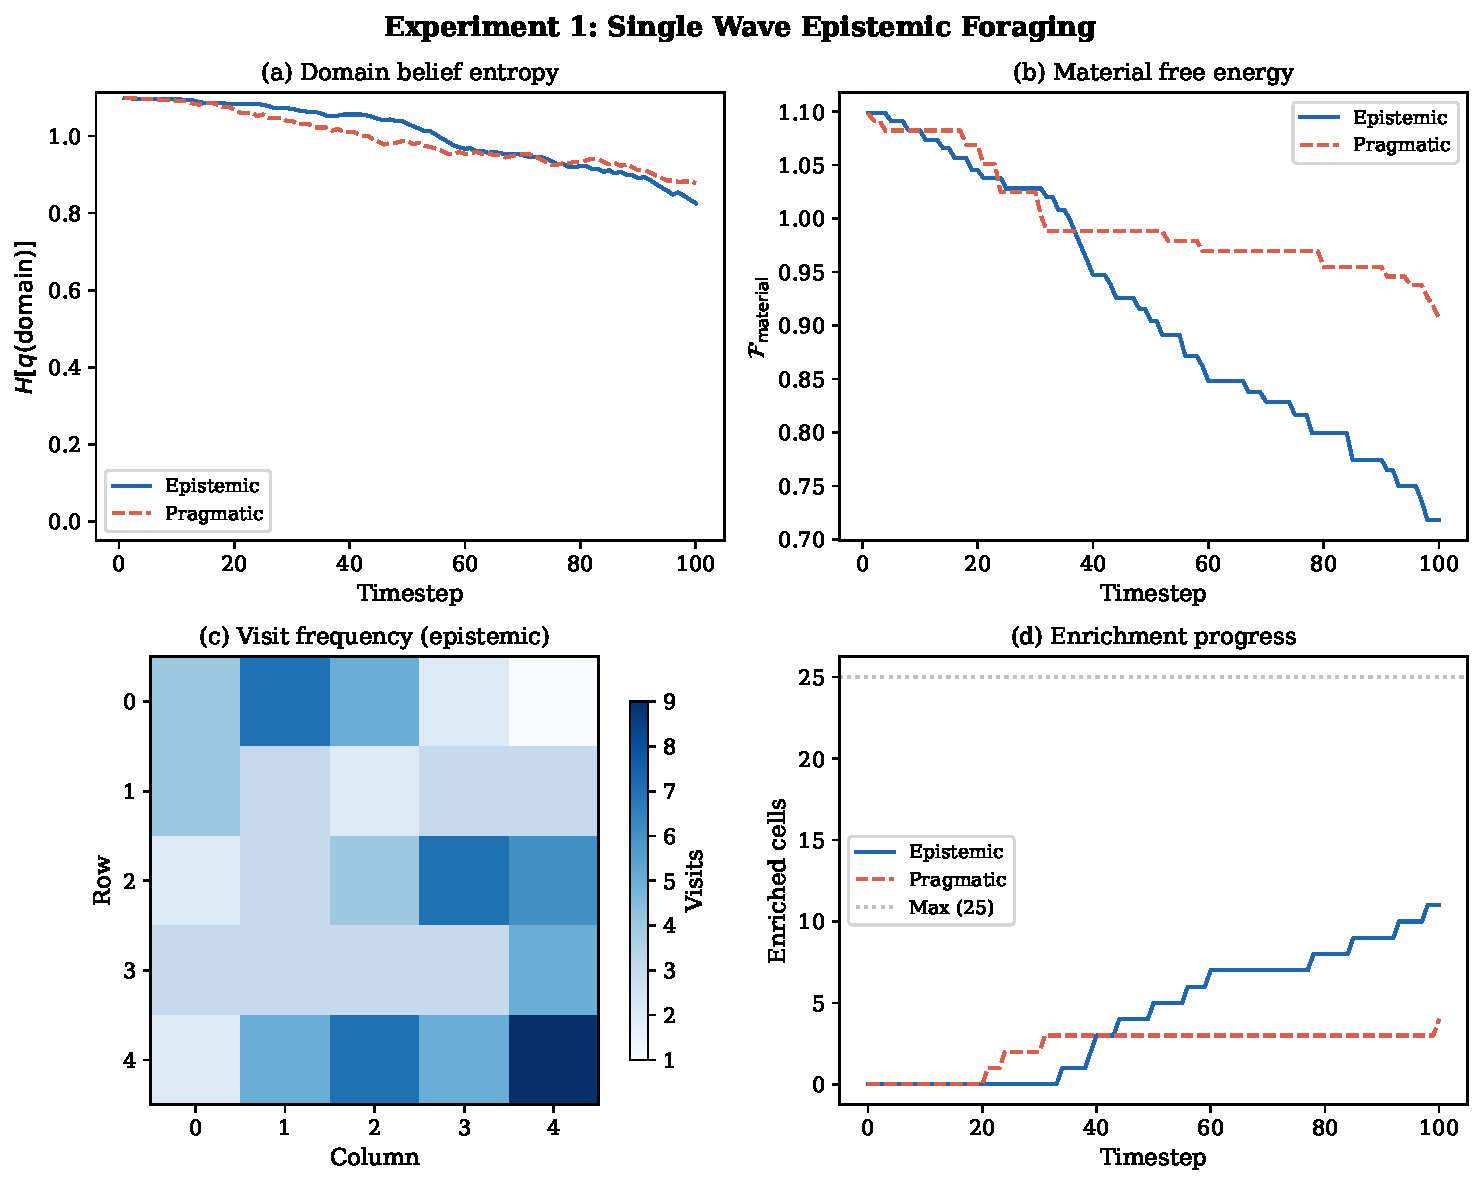
\includegraphics[width=\textwidth]{figures/exp1_epistemic_foraging.pdf}
\caption{Single Wave epistemic foraging on the semiotic fabric. (a)~Domain belief entropy decreases as the Wave accumulates evidence. (b)~Material free energy $\mathcal{F}_{\text{material}}$ converges faster with epistemic drive (two-step EFE). (c)~Visit frequency heatmap shows systematic exploration. (d)~Enrichment progress: epistemic Wave enriches $2.75\times$ more cells than the pragmatic-only baseline.}
\label{fig:exp1}
\end{figure}

\begin{figure}[H]
\centering
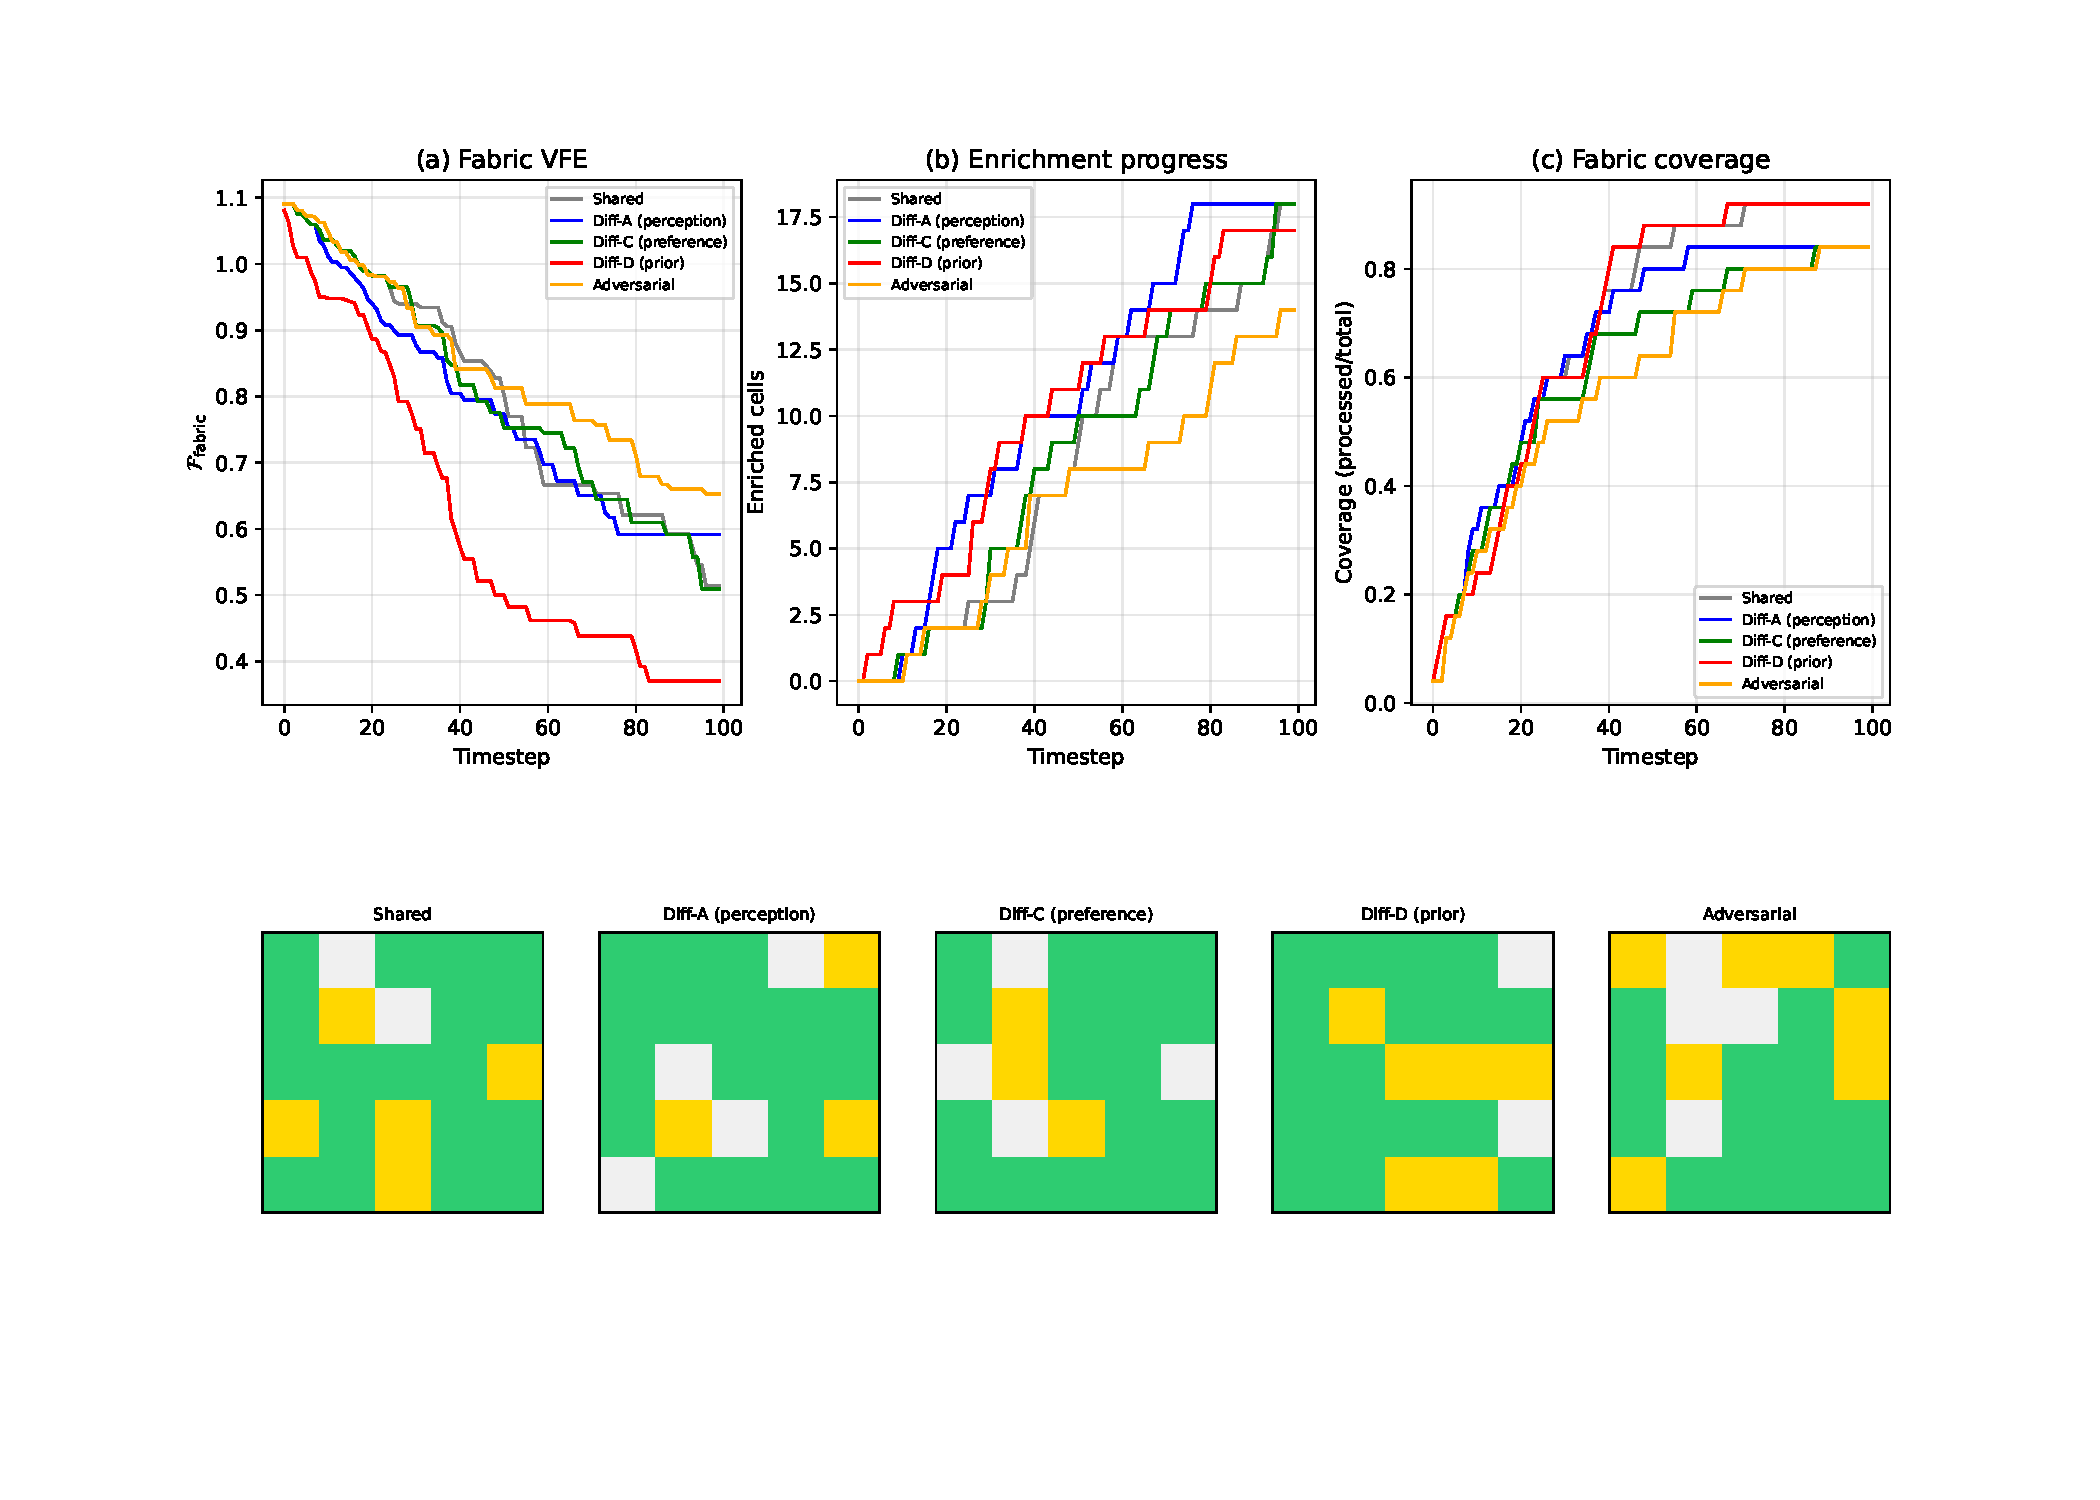
\includegraphics[width=\textwidth]{figures/exp2_multiwave_cooperation.pdf}
\caption{Isolating generative model component contributions to multi-Wave cooperation. Top row: (a)~Material free energy over time for five conditions isolating $\mathbf{A}$, $\mathbf{C}$, and $\mathbf{D}$ matrix differentiation. (b)~Enrichment progress. Bottom row: final enrichment state heatmaps for each condition, showing how different forms of generative model heterogeneity produce distinct spatial coverage patterns. Diff-D achieves lowest $\mathcal{F}_{\text{material}}$; adversarial performs worst due to complete model misspecification.}
\label{fig:exp2}
\end{figure}

\begin{figure}[H]
\centering
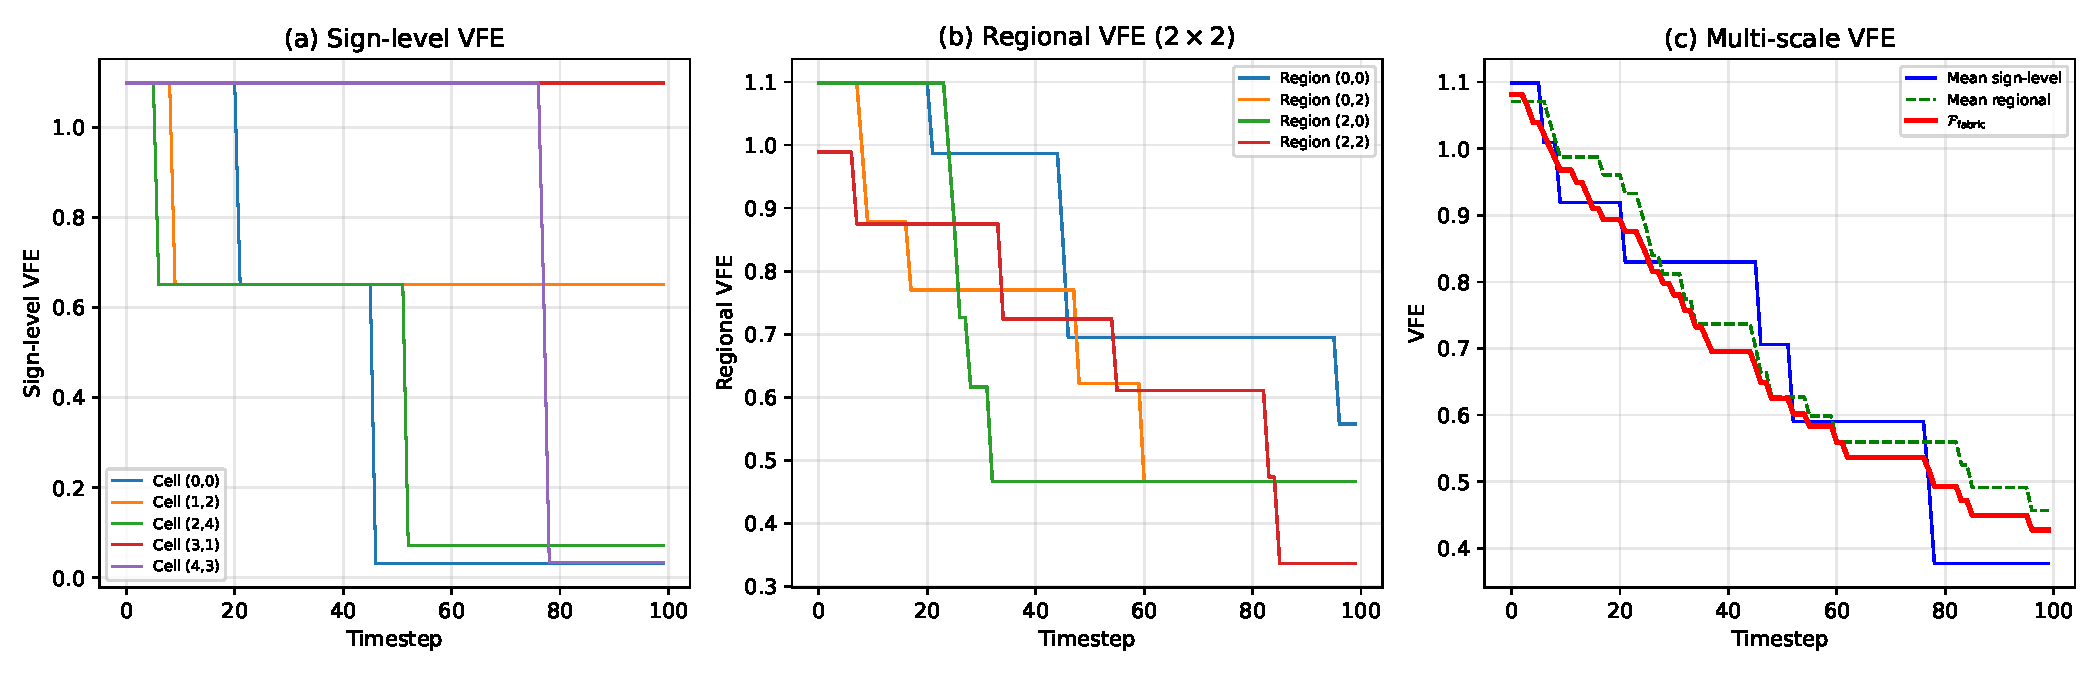
\includegraphics[width=\textwidth]{figures/exp3_nested_free_energy.pdf}
\caption{Nested free energy minimization across Markov blanket levels. (a)~Sign-level $F$ shows variability as individual cells are enriched. (b)~Regional ($2 \times 2$) free energy smooths individual fluctuations. (c)~Fabric-level $\mathcal{F}_{\text{material}}$ integrates across all scales, showing monotonic decrease.}
\label{fig:exp3}
\end{figure}


% ============================================================
% 6. IMPLICATIONS AND APPLICATIONS
% ============================================================
\section{Implications and Applications}
\label{sec:implications}

\subsection{For Active Inference Theory}

SemApp provides what may be the first operational, production-scale instantiation of nested Markov blankets in a computational system. While the theory of nested blankets has been developed extensively in the context of biological systems \citep{friston2019particular, kirchhoff2018markov, ramstead2023inner}, its application to engineered data systems is novel. The SemApp deployment at NGA --- processing petabytes of data with hundreds of concurrent users over nearly a decade --- constitutes an empirical test bed for nested blanket theory at a scale unprecedented in the literature.

The Peirce--FEP isomorphism (Proposition~\ref{prop:peirce}) suggests that semiotics is not merely an analogy for active inference but a \emph{consequence} of the FEP applied to sign systems. If this isomorphism holds as strongly as the formal analysis suggests, then any system performing active inference over meaningful content is, by definition, performing semiosis. This has implications for the biosemiotics literature, which has independently argued that life is a semiotic process.

The multi-Wave dynamics of the PWF provide a test bed for the epistemic community theory of \citet{albarracin2022epistemic}. Experiment 2 demonstrates that Wave ecosystems exhibit the same dynamics as social epistemic communities: each generative model component ($\mathbf{A}$, $\mathbf{C}$, $\mathbf{D}$) contributes a distinct mechanism to collective sense-making---perceptual expertise, goal-directed spatial specialization, and prior-dependent enrichment success, respectively---while complete model misspecification (adversarial condition) degrades fabric quality. This opens the possibility of engineering Wave ecosystems with designed epistemic properties.

We note the connection to the minimal sentience framework of \citet{hipolito2025beyond}, which proposes three conditions: active self-maintenance, historical adaptability, and autonomous agency. SemApp's fabric demonstrably satisfies the first two (self-maintenance through continuous processing and fault tolerance; historical adaptability through fingerprints and provenance). Whether it satisfies autonomous agency --- whether Wave processing constitutes genuine action initiation rather than triggered response --- is a theoretical question that merits further investigation.

\subsection{For DoD/IC Data Architecture}

The active inference framework provides predictive design principles for next-generation data architectures:

\begin{enumerate}[nosep]
    \item \textbf{Epistemic diversity}: Theorem~\ref{thm:nested_blanket} and Experiment 2 predict that diverse Wave ecosystems outperform homogeneous ones. Data architectures should encourage third-party Wave development rather than centralizing processing in a small number of pipelines.

    \item \textbf{Classification as blanket integrity}: Security classification is not overhead --- it is a necessary component of Markov blanket maintenance (Equation~\ref{eq:ci}). Weakening classification controls would compromise the conditional independence that enables modular processing.

    \item \textbf{Provenance as cognitive memory}: Fingerprints and Perceiver metadata are not merely compliance mechanisms --- they provide the non-Markovian temporal depth necessary for genuine sense-making (Section~\ref{sec:waves}). Systems that discard provenance are amnesic.

    \item \textbf{$\mathcal{F}_{\text{material}}$ as health metric}: The material free energy provides a principled, scalar metric for operational monitoring. A real-time $\mathcal{F}_{\text{material}}$ dashboard would give operators visibility into the fabric's sense-making capacity.

    \item \textbf{Domain models as adaptive priors}: Layer 3 should be treated as a space of priors that can be updated through experience, not as a fixed schema. This aligns with SemApp's existing approach of making standardization optional rather than mandatory.
\end{enumerate}

\subsection{Designing Explainable Semiotic AI}

\citet{albarracin2023explainable} argue that active inference systems with explicit generative models are inherently explainable: every action can be traced to a belief, every belief to an observation, and every observation to a specific element of the generative model. Applied to SemApp, this means every Wave enrichment can be explained via its DEEP decomposition:

\begin{itemize}[nosep]
    \item ``This enrichment was made because the classification policy required it'' (Deontic)
    \item ``This enrichment was made because it resolved uncertainty about the Sign's referent'' (Epistemic)
    \item ``This enrichment was made because it moved the fabric closer to domain model conformance'' (Pragmatic)
    \item ``This enrichment was made because the domain model predicts this Concept for this Signifier'' (Preferential)
\end{itemize}

Combined with fingerprint provenance and the fabric's full enrichment history, this provides explainability by construction --- not as a post-hoc add-on but as an architectural property of active inference systems.


% ============================================================
% 7. DISCUSSION
% ============================================================
\section{Discussion}
\label{sec:discussion}

\subsection{Limitations}

The formal mapping presented in this paper is \emph{structural}: we show that SemApp's architecture has the form of a nested Markov blanket system performing active inference. We do not claim that SemApp was designed with the FEP in mind (it was not), nor that its developers intended to implement active inference. Rather, we argue that the architecture converged on an FEP-consistent design because the FEP describes the necessary conditions for any system that maintains its organization while making sense of a complex environment. This convergent design is, if anything, stronger evidence for the framework's explanatory power than a design that deliberately instantiated FEP principles.

The pymdp simulation is a proof of concept, not a model of SemApp at operational scale. The $5 \times 5$ grid with 3 semantic states is many orders of magnitude smaller than SemApp's actual state space ($\sim 70$ PB of data across millions of Signs). Scaling the simulation to realistic dimensions would require approximate inference methods beyond the scope of this paper.

The conditional independence claim in Theorem~\ref{thm:nested_blanket} holds at the architectural level (by design, Artifacts and domain models interact only through Signs), but could be violated in practice by side channels (e.g., file naming conventions that leak domain model information into Layer 1). A formal verification of blanket integrity in the running system is an open challenge.

\subsection{Future Directions}

Several lines of future work emerge from this analysis:

\begin{enumerate}[nosep]
    \item \textbf{Online $\mathcal{F}_{\text{material}}$ monitoring}: Implementing a real-time computation of the fabric's material free energy would provide an operational metric for the fabric's sense-making capacity. This requires efficient approximation methods, since exact computation is intractable.

    \item \textbf{Wave design as generative model engineering}: If Waves are active inference agents, then designing Waves is designing generative models. The DEEP decomposition provides a principled framework for specifying what a Wave should seek (epistemic value), what it should achieve (pragmatic value), and what constraints it should respect (deontic value).

    \item \textbf{Multi-fabric federation as distributed active inference}: SemApp supports distributed query across instances. Under our framework, this corresponds to distributed active inference across organizational Markov blankets --- a formal model for inter-agency information sharing.

    \item \textbf{Adversarial robustness as blanket defense}: Data poisoning and adversarial injection can be understood as attacks on Markov blanket integrity. The FEP provides a principled framework for detecting and defending against such attacks: anomalous increases in $\mathcal{F}_{\text{material}}$ signal blanket violation.

    \item \textbf{Connection to the Ecosystem of Intelligence vision}: \citet{friston2022ecosystems} propose engineering ecosystems of natural and artificial intelligence through shared generative models. SemApp's fabric, with its unified API and Wave framework, provides a concrete substrate for such ecosystems.
\end{enumerate}


% ============================================================
% 8. CONCLUSION
% ============================================================
\section{Conclusion}
\label{sec:conclusion}

We have argued that the SemApp semiotic data fabric is not merely a data platform but a cognitive substrate --- a system that satisfies the formal criteria for cognition under the Free Energy Principle. The argument rests on three pillars:

First, \textbf{semiosis is inference}. The Peirce--FEP isomorphism (Proposition~\ref{prop:peirce}, Theorem~\ref{thm:semiotic_fe}) establishes that Sign creation in SemApp --- binding Signifiers with Concepts --- is variational inference that minimizes semiotic free energy. The fabric does not merely store data; it \emph{interprets} it, generating meaning through the same formal process that defines cognition under the FEP.

Second, \textbf{the architecture is a nested Markov blanket system} (Theorem~\ref{thm:nested_blanket}). The three-layer architecture, with Artifacts as external states, Signs as blanket states, and domain models as internal states, satisfies the conditional independence requirements of the blanket partition. Each Sign has its own blanket nested within the layer blanket, nested within the fabric blanket --- the recursive structure that \citet{kirchhoff2018markov} identify as the hallmark of cognitive systems.

Third, \textbf{Process Waves are active inference agents} (Definition~\ref{def:wave_gm}) that coordinate through shared Markov blankets (Proposition~\ref{prop:shared}), creating the network effect that makes the fabric progressively more capable. The material free energy $\mathcal{F}_{\text{material}}$ (Definition~\ref{def:f_material}) provides a principled metric for this progressive sense-making, and its monotonic decrease (Proposition~\ref{prop:monotone}) under consistent processing constitutes the fabric's learning.

The computational demonstration validates this framework: a pymdp simulation shows that active inference agents on a semiotic grid exhibit epistemic foraging, cooperative dynamics, and multi-scale free energy minimization --- the signatures of a cognitive system.

Nearly a decade of operational experience at NGA, processing tens of petabytes of data and supporting mission-critical intelligence operations, provides empirical validation at a scale unprecedented for nested Markov blanket theory. The framework not only explains why SemApp works but predicts how to extend it: through epistemic Wave diversity, adaptive domain models, and $\mathcal{F}_{\text{material}}$ monitoring.

We believe this analysis opens a door to a new class of data architectures --- \emph{cognitive data fabrics} --- that are designed from first principles to make sense of the world. In the spirit of \citet{friston2022ecosystems}, such fabrics may form the substrate for ecosystems of intelligence in which humans, algorithms, and institutions coordinate through shared semiotic structures, achieving collective sense-making at the scale that the challenges of the 21st century demand.


% ============================================================
% REFERENCES
% ============================================================
\bibliographystyle{apalike}

\begin{thebibliography}{99}

\bibitem[Albarracin(2023)]{albarracin2023archaeological}
Albarracin, M. (2023).
\newblock Integrating Active Inference and New Materialism in Archaeological Interpretation.
\newblock \emph{PNAS Nexus}.

\bibitem[Albarracin(2023b)]{albarracin2023embodiment}
Albarracin, M. (2023).
\newblock Cultural bodybuilding: The embodied influence of culture on perception and action.
\newblock In \emph{Embodied Cognition and Active Inference}.

\bibitem[Albarracin(2026)]{albarracin2026empathy}
Albarracin, M. (2026).
\newblock Empathy modeling in active inference agents via the prisoner's dilemma.
\newblock Manuscript.

\bibitem[Albarracin \& Sakthivadivel(2025)]{albarracin2025nonmarkovian}
Albarracin, M. \& Sakthivadivel, D.~A.~R. (2025).
\newblock Non-{M}arkovian systems, phenomenology, and the challenges of capturing meaning and context --- {C}omment on {P}arr, {P}ezzulo, and {F}riston (2025).
\newblock Letter submitted to \emph{JSEDI}.

\bibitem[Albarracin et~al.(2021)]{albarracin2021variational}
Albarracin, M., Constant, A., Friston, K.~J., \& Ramstead, M.~J.~D. (2021).
\newblock A variational approach to scripts.
\newblock \emph{Frontiers in Psychology}, 12, 585493.

\bibitem[Albarracin et~al.(2022)]{albarracin2022epistemic}
Albarracin, M., Demekas, D., Ramstead, M.~J.~D., \& Heins, C. (2022).
\newblock Epistemic communities under active inference.
\newblock \emph{Entropy}, 24(4), 476.

\bibitem[Albarracin et~al.(2023c)]{albarracin2023explainable}
Albarracin, M., Hip\'{o}lito, I., Essafi~Tremblay, S., Fox, J.~G., Ren\'{e}, G., Friston, K.~J., \& Ramstead, M.~J.~D. (2023).
\newblock Designing explainable {AI} with active inference.
\newblock \emph{arXiv preprint}, 2305.02205.

\bibitem[Bouizegarene et~al.(2023)]{bouizegarene2023narrative}
Bouizegarene, N., Ramstead, M.~J.~D., Constant, A., Friston, K.~J., \& Kirmayer, L.~J. (2023).
\newblock Narrative as active inference: An integrative account of the functions of narratives.
\newblock \emph{Psychological Review}.

\bibitem[Constant et~al.(2019)]{constant2019regimes}
Constant, A., Ramstead, M.~J.~D., Veissi\`{e}re, S.~P.~L., \& Friston, K.~J. (2019).
\newblock Regimes of expectations: An active inference model of social conformity and human decision making.
\newblock \emph{Frontiers in Psychology}, 10, 679.

\bibitem[Fields et~al.(2025)]{fields2025inner}
Fields, C., Albarracin, M., Friston, K.~J., Kiefer, A., Ramstead, M.~J.~D., \& Safron, A. (2025).
\newblock The inner screen model of consciousness.
\newblock \emph{Neuroscience of Consciousness}, niaf009.

\bibitem[Friston(2019)]{friston2019particular}
Friston, K.~J. (2019).
\newblock A free energy principle for a particular physics.
\newblock \emph{arXiv preprint}, 1906.10184.

\bibitem[Friston et~al.(2022)]{friston2022ecosystems}
Friston, K.~J., Ramstead, M.~J.~D., Kiefer, A.~B., Tschantz, A., Buckley, C.~L., Albarracin, M., \ldots~Ren\'{e}, G. (2022).
\newblock Designing ecosystems of intelligence from first principles.
\newblock \emph{arXiv preprint}, 2212.01354.

\bibitem[Gu\'{e}nin-Carlut \& Albarracin(2023)]{guenincarlut2023embedded}
Gu\'{e}nin-Carlut, A. \& Albarracin, M. (2023).
\newblock On embedded normativity: An active inference account of agency beyond flesh.
\newblock In \emph{Active Inference Workshop}, Springer.

\bibitem[Heins et~al.(2022)]{heins2022pymdp}
Heins, C., Millidge, B., Da~Costa, L., et~al. (2022).
\newblock pymdp: A {P}ython library for active inference in discrete state spaces.
\newblock \emph{Journal of Open Source Software}, 7(73), 4098.

\bibitem[Hip\'{o}lito et~al.(2025)]{hipolito2025beyond}
Hip\'{o}lito, I., Albarracin, M., \& Hynes, J.~B. (2025).
\newblock Beyond imitation games: A falsifiable emergent sentience framework.
\newblock Manuscript.

\bibitem[Kirchhoff et~al.(2018)]{kirchhoff2018markov}
Kirchhoff, M.~D., Parr, T., Palacios, E., Friston, K.~J., \& Kiverstein, J. (2018).
\newblock The {M}arkov blankets of life: Autonomy, active inference and the free energy principle.
\newblock \emph{Journal of the Royal Society Interface}, 15(138), 20170792.

\bibitem[Parr et~al.(2022)]{parr2022active}
Parr, T., Pezzulo, G., \& Friston, K.~J. (2022).
\newblock \emph{Active Inference: The Free Energy Principle in Mind, Brain, and Behavior}.
\newblock MIT Press.

\bibitem[Pattisapu et~al.(2024)]{pattisapu2024circumplex}
Pattisapu, V., Verbelen, T., Pitliya, R., Kiefer, A., \& Albarracin, M. (2024).
\newblock Free energy in a circumplex model of emotion.
\newblock \emph{VERSES Research Lab}.

\bibitem[Peirce(1931)]{peirce1931collected}
Peirce, C.~S. (1931--1958).
\newblock \emph{Collected Papers of Charles Sanders Peirce} (Vols.~1--8).
\newblock Harvard University Press.

\bibitem[Ramstead et~al.(2016)]{ramstead2016cultural}
Ramstead, M.~J.~D., Veissi\`{e}re, S.~P.~L., \& Kirmayer, L.~J. (2016).
\newblock Cultural affordances: Scaffolding local worlds through shared intentionality and regimes of attention.
\newblock \emph{Frontiers in Psychology}, 7, 1090.

\bibitem[Ramstead et~al.(2023)]{ramstead2023inner}
Ramstead, M.~J.~D., Albarracin, M., Kiefer, A., Klein, B., Fields, C., Friston, K.~J., \& Safron, A. (2023).
\newblock Steps towards a minimal unifying model of consciousness.
\newblock \emph{arXiv preprint}, 2306.04025.

\bibitem[SEI(2006)]{sei2006uls}
Feiler, P. et~al. (2006).
\newblock \emph{Ultra-Large-Scale Systems: The Software Challenge of the Future}.
\newblock Software Engineering Institute, Carnegie Mellon University.

\bibitem[Veissi\`{e}re et~al.(2020)]{veissiere2020thinking}
Veissi\`{e}re, S.~P.~L., Constant, A., Ramstead, M.~J.~D., Friston, K.~J., \& Kirmayer, L.~J. (2020).
\newblock Thinking through other minds: A variational approach to cognition and culture.
\newblock \emph{Behavioral and Brain Sciences}, 43, e90.

\bibitem[Yoakum-Stover \& Eick(2025)]{yoakumstover2025semapp}
Yoakum-Stover, S. \& Eick, M.~A. (2025).
\newblock The {SemApp} data fabric.
\newblock \emph{Mission Focus White Paper}.

\end{thebibliography}


% ============================================================
% APPENDICES
% ============================================================
\appendix

\section{Proof of the Nested Blanket Theorem}
\label{app:proof}

We provide the full proof of Theorem~\ref{thm:nested_blanket}.

\begin{proof}
We must show that $\bp(\mathcal{X}_1, \mathcal{X}_3 | \mathcal{X}_2) = \bp(\mathcal{X}_1 | \mathcal{X}_2) \cdot \bp(\mathcal{X}_3 | \mathcal{X}_2)$; that is, Artifact states and domain model states are conditionally independent given Sign states.

\textbf{Step 1: Characterize information flow.} In the SemApp architecture, information flows as follows:
\begin{itemize}[nosep]
    \item Artifacts $\to$ Signs: via Ingest (creating Artifact records) and Digest Waves (extracting Signs from Artifact content, linked by Mentions)
    \item Signs $\to$ Domain Models: via Layer 3 assertions (Signs instantiate Concepts defined in domain models)
    \item Domain Models $\to$ Signs: via Concept definitions (domain models define the vocabulary of Concepts available for Sign creation)
    \item Signs $\to$ Artifacts: via Reification and enrichment (Signs reference Artifacts through Mentions)
\end{itemize}

\textbf{Step 2: Verify no direct Artifact--Domain Model pathway.} By architectural specification:
\begin{itemize}[nosep]
    \item Artifacts contain no domain model references (they are raw files with metadata: address, size, type, classification)
    \item Domain models contain no Artifact references (they define Concepts, predicates, and ontological relations abstractly)
\end{itemize}
Any correlation between an Artifact's content and a domain model's structure is mediated by the Signs extracted from that Artifact using that domain model's Concepts. Formally:
\begin{equation}
\bp(x_1 \in \mathcal{X}_1, x_3 \in \mathcal{X}_3) = \sum_{x_2 \in \mathcal{X}_2} \bp(x_1 | x_2) \cdot \bp(x_3 | x_2) \cdot \bp(x_2)
\end{equation}

\textbf{Step 3: Identify blanket decomposition.} Within Layer 2:
\begin{itemize}[nosep]
    \item Sensory states $\bs$: Signifiers and Mentions carry information \emph{from} the external world. A Signifier is a data value extracted from an Artifact; a Mention points back to the source. These states are influenced by external states (Artifacts) but do not directly influence them.
    \item Active states $\ba$: Associations, Context links, and Reification impose structure \emph{on} the fabric. An Association asserts a relation visible to other Waves and applications. These states influence the external environment (by making the fabric more discoverable and useful) without being directly influenced by it.
\end{itemize}

\textbf{Step 4: Verify conditional independence.} Given the Sign states (Layer 2):
\begin{align}
\bp(\text{Artifact content} | \text{Signs}, \text{Domain Models}) &= \bp(\text{Artifact content} | \text{Signs}) \\
\bp(\text{Domain structure} | \text{Signs}, \text{Artifacts}) &= \bp(\text{Domain structure} | \text{Signs})
\end{align}
The first holds because knowing the Signs (which include all extracted information from the Artifact via Mentions) d-separates the Artifact content from the domain model. The second holds because knowing the Signs (which instantiate the domain model's Concepts) d-separates the domain model structure from the Artifact content. \qed
\end{proof}


\section{Glossary: SemApp--Active Inference Terminology Mapping}
\label{app:glossary}

\begin{table}[H]
\centering
\caption{Mapping between SemApp and Active Inference terminology}
\begin{tabular}{lll}
\toprule
\textbf{SemApp Term} & \textbf{Active Inference Term} & \textbf{Formal Symbol} \\
\midrule
Artifact & Observation / sense data & $\bo$ \\
Sign & Variational belief (interpretant) & $\bq_\sigma(s)$ \\
Signifier & Sensory state & $\bs$ \\
Concept & Internal state / posterior mode & $\bmu$ \\
Association & Factor graph edge & $\bp(s_j | s_i, \text{pred})$ \\
Reification & Hierarchical belief & $\bq^{(\ell+1)}$ \\
Domain Model & Generative model prior & $\bp(\bs)$ \\
Process Wave & Active inference agent & Agent($\mathbf{A}, \mathbf{B}, \mathbf{C}, \mathbf{D}$) \\
Fingerprint & Action trace / memory & $\bpi_{\text{history}}$ \\
Enrichment & Active state / action & $\ba$ \\
Classification Label & Deontic cue & $c_{\text{deontic}}$ \\
Perceiver & Provenance / trust weight & $\omega_{\text{precision}}$ \\
Layer 1 (Artifacts) & External states & $\boldeta$ \\
Layer 2 (Signs) & Blanket states & $\mathcal{B} = \bs \cup \ba$ \\
Layer 3 (Models) & Internal states & $\bmu$ \\
Network Effect & Shared Markov blanket & $\mathcal{S}_{\text{shared}}$ \\
$\mathcal{F}_{\text{material}}$ & Fabric free energy & $\mathcal{F}_{\text{material}}$ \\
\bottomrule
\end{tabular}
\end{table}


\end{document}
